
\chapter[Ausblick ]{Ausblick} \label{Kapitel6}

\section*{Rückblick}

In der Einleitung, Kapitel~\vref{Kapitel1}, wurden zwei Beispiele für Moving--Regions gegeben und die Frage gestellt, ob es gelingen würde aus diesen Unwetter--Daten beziehungsweise den DETER--Daten kontinuierliche Bewegungen zu erzeugen. 

Zum ersten Beispiel kann nun gesagt werden, dass die Erzeugung prinzipiell gelingen würde (Falls das Beispiel nicht ein komplett fiktives wäre.). Jedoch würden bei Wetterdaten, die stark rotierende Daten sind die Probleme aus ~\vref{ProblemeRotation} zum Tragen kommen. In Abbildung~\vref{fig:Wetterdaten} wurde versucht, den Charakter von sich bewegenden Luftdruckgebieten zu treffen. Man kann gut sehen, dass die Interpolation zwar gelingt, das Ergebnis nach der Hälfte der Zeit aber viel zu groß ist und den beiden \textit{Faces} nicht stark ähnelt.

\begin{figure}
	\centering
	\includegraphics[scale=0.8]{Wetterdaten.eps}
	\caption[Bewegende Wetterdaten]{Fiktives Beispiel für bewegende Wetterdaten\\\textit{Quelle: Eigene Darstellung}}
	\label{fig:Wetterdaten}
\end{figure}
Beim zweiten Beispiel, den DETER--Daten, ist Überführung der Daten in eine kontinuierliche Form möglich, wie in Kapitel~\vref{Kapitel5} geschehen.


Auf dem Weg zur Lösung dieser Probleme wurden zwei verschiedene Applikationen erzeugt, das Java--Applet und die SECONDO--Algebra. 
Die Java-Applikation entstand nur aufgrund der Tatsache, dass es bereits eine solche Applikation gab, die von Erlend T\o{}ssebro entwickelt worden war. Diese Applikation wurde von dem Autor dieser Arbeit erweitert, so dass diese nun die Problemstellung der Arbeit löst. Obwohl diese Applikation nicht gefordert war, ist dieses Programm nicht überflüssig, es zeigt didaktisch gut aufbereitet wie das Matching passiert.

Die SECONDO--Algebra integriert die Möglichkeit zur Berechnung von kontinuierlichen Bewegungen in das SECONDO--System. Innerhalb dieses System ist es nun also möglich Regionen zu interpolieren. Aus technischen Gründen wurde dieser eine Operator als eigene Algebra implementiert, eine spätere Integration dieses Operators in die Moving--Region--Algebra ist aber möglich.




\section*{Probleme}
Sowohl bei der Bestimmung von Matchings mittels des Overlapping--Matches, als auch bei der Berechnung der entsprechenden Overlap--Bewertung, wird die Intersection--Funk"-tion der MakeOp-Klasse verwendet. Diese findet sich in der Plane--Sweep--Algebra. Leider führte die Verwendung dieser Funktion immer wieder zu Abstürzen, wie sie auch bei der Verwendung des \textit{union\_new} Operators derselben Algebra auftauchen. Deshalb wurde es leider nötig, auf diese Verfahren zu verzichten. Wenn die Probleme mit der externen Algebra behoben sind, kann man diese Verfahren einfach wieder reaktivieren, indem man in der Datei ,,RegionInterpolator.h'' die folgende Zeile wieder einkommentiert.
\begin{verbatim}
#define USE_OVERLAP
\end{verbatim}  

\section*{Erfahrungen}

In \vref{Zerlegung} wurde ein Algorithmus vorgestellt, der ein Polygon in konvexe Polygone zerlegen kann. Der Algorithmus wurde in der Hoffnung entwickelt, eine wesentlich weniger kleinteilige Zerlegung der Polygone zu erreichen, als das eine Triangulierung liefern würde. In der praktischen Erfahrung zeigt sich aber, dass die Zerteilung bei realen, komplizierten \textit{Faces} mit \textit{Holes} doch sehr kleinteilig wird. Abbildung~\vref{fig:ZerlegungFace2} zeigt ein solches Beispiel.

Die Verwendung dieses Algorithmus kann deshalb nicht uneingeschränkt empfohlen werden. Falls nicht klar ist, wie kompliziert die zu zerlegenden Polygone aufgebaut sind, so empfiehlt sich eher die Verwendung eines performanten Triangulierungs--Algorithmus. Ein solcher Algorithmus wird etwa unter \cite{Sei} vorgestellt.


\begin{figure}
	\centering
	\includegraphics[scale=0.9]{Convexer.svg.eps}
	\caption[Zerlegung eines Polygons, nur wenig besser als eine Triangulierung]{Ein Beispiel, in dem die Zerlegung eines Polygons Zerlegung liefert, die kaum besser als eine Triangulierung ist. Ein einziges Viereck ist das einzige vorkommende Polygon, das kein Dreieck ist.\\\textit{Quelle: Eigene Darstellung}}
	\label{fig:ZerlegungFace2}
\end{figure}

\section*{Raum für weitere Überlegungen}

Obwohl die implementierten Matchings bereits gute Ergebnisse liefern, kann man die entsprechende SECONDO--Algebra als Framework begreifen, um andere vielversprechende Matchings zu implementieren. Bei der Imlementierung der Algebra wie auch der Java--Applikation wurde auf eine guter Erweiterbarkeit geachtet, so dass eine Implementierung komplexerer Matching-Verfahren mit geringem Aufwand möglich ist. Es erscheint durchaus empfehlenswert, die eigenen Ideen zuerst in der Java--Applikation zu entwickeln, da diese viele Möglichkeiten des optischen Debuggen bietet. Im Anhang~\vref{eigeneMatch} wird beschrieben, wie man eigene Verfahren zum Matchen und Bewerten  implementieren, und wie man diese Verfahren in die Algebra einbauen kann.

Im Laufe der Arbeit wurden bereits einige Verfahren aufgezeigt, die eventuell gute Matches liefern können:
\begin{itemize}
\item Algorithmen zum Finden von pseudooptimalen Lösungen

In \vref{AARR} und \vref{AFRWW} wurden die Algorithmen aus den Veröffentlichungen \cite{AAR} und \cite{AFRW} vorgestellt. Diese Algorithmen könnten sehr gute Ergebnisse mit vertretbaren Aufwänden liefern. Da diese Paper aber eher aus dem Bereich der Mustererkennungen kommen, kümmern sich diese nur um 1:1 Matches.  Wie man mit diesen Algorithmen auf Vereinigungen und Zersplitterungen reagieren kann, muss noch überlegt werden.

\item Bewertung mittels $\min_{T\in\mathcal{T}}\delta(A,T(B))$

Das Verfahren, welches im letzten Abschnitt beschrieben wurde, liefert auch die Möglichkeit, gegebene 1:1 Matches zu bewerten. Eine diesbezügliche Implementierung wird voraussichtlich gute Ergebnisse bieten. 

\item statistisches Referenzpunktverfahren

In \vref{StatistikAlgo} wurde ein Verfahren aufgezeigt, das mittels statistischer Analyse aus einer Menge von Referenzpunkten zusammengehörige Cluster finden kann. Möglicherweise könnte dieses Verfahren gute Ergebnisse liefern, die Laufzeit wird aber nicht besonders gut sein.

\item Verfahren mit neuronalen Netzen oder mit Support--Vector--Maschinen

Unter \vref{neuroNetz} wurde auch ein Verfahren andiskutiert, das eine Gruppenbildung auf einer Menge von Referenzpunkten mittels neuronaler Netze oder Support--Vector--Maschinen durchführt. Weitere Überlegungen in dieser Richtung, zu Laufzeiten oder Qualitäten, wurden nicht angestellt. 
 
\item Maximize Overlap (set of cycles)

In \cite{TG} wird ein Matching--Verfahren entwickelt, das zwei Flächen matched, wenn Ihre Überlappung maximal ist. Dieses Verfahren ist unter Kapitel~\vref{MaxOver} näher beschrieben. Auch dieses Verfahren wurde nicht implementiert, könnte aber zu interessanten Ergebnissen führen.
\end{itemize}



